
%(BEGIN_QUESTION)
% Copyright 2015, Tony R. Kuphaldt, released under the Creative Commons Attribution License (v 1.0)
% This means you may do almost anything with this work of mine, so long as you give me proper credit

Examine this schematic diagram sampled from Victor H. Todd's 1922 book {\it Protective Relays} showing a very simple protection circuit comprised of a power circuit breaker with an externally energized ``trip coil'', a current transformer, a DC storage battery, and a ``plunger-style'' protective relay:

$$\epsfxsize=6in 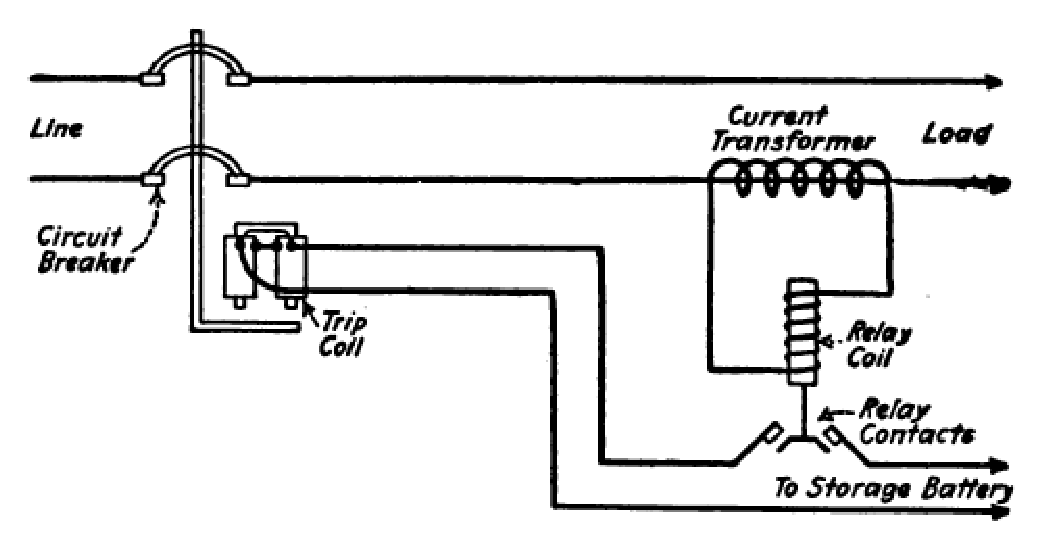
\includegraphics[width=15.5cm]{i02862x01.eps}$$

First, identify the purpose of this protective system.  What abnormal condition is it designed to sense, and how does it protect the system against damage from this abnormal condition?

\vskip 10pt

Suppose this relay has been calibrated to ``pick up'' at a current transformer output of 3.2 amps AC.  If the current transformer's ratio is 800:5, how many amps of line current does this represent?

%One of the important tasks of a protective relay technician is to routinely check the calibration of protective relays to ensure they will act at precisely the correct moment.  Identify how the ``pickup'' value (i.e. the trip threshold) for this legacy design of protective relay could be checked against a calibration standard by a technician.  Remember, this is 1922 and we don't have digital multimeters at our disposal!

\vskip 10pt

Finally, identify how the ``pickup'' value (i.e. the trip threshold) for this protective relay might be adjusted by a technician.

\vskip 20pt \vbox{\hrule \hbox{\strut \vrule{} {\bf Suggestions for Socratic discussion} \vrule} \hrule}

\begin{itemize}
\item{} Which ANSI number code best corresponds to this particular protective relay function?  How can you tell?
\item{} Suppose the storage battery became discharged so that it measured only about 90 volts rather than 120 volts.  How would this affect the operation of this protective system, if at all?
\item{} Suppose the current transformer failed with an internally shorted winding, so that its effective turns ratio became closer to being 1:1 than it is now.  How would this affect the operation of this protective system, if at all?
\item{} Two important concepts are used in the electric power industry to express the reliability of the system: {\it dependability} and {\it security}.  Dependability is the likelihood that a protective device or system will shut off power as designed in the event of an fault.  Security is the likelihood that a protective device will allow power to remain on when there is no fault (i.e. the likelihood it will not needlessly trip).  Identify a specific fault in this protective system that could compromise its dependability, and another specific fault that could compromise its security.
\end{itemize}

\underbar{file i02862}
%(END_QUESTION)





%(BEGIN_ANSWER)

\noindent
{\bf Partial answer:}

\vskip 10pt

This is an {\it instantaneous overcurrent} relay, corresponding to ANSI function code {\it 50}.
 
%(END_ANSWER)





%(BEGIN_NOTES)

This system senses line current, causing the plunger-style relay to ``pick up'' if the current exceeds a pre-set value.  Once picked up, the relay sends a DC signal to the circuit breaker's trip coil, causing that breaker to trip open and interrupt fault current on the power system.

\vskip 10pt

A current transformer ratio of 800:5 is equivalent to 160:1, which means for every 1 amp of current delivered to the relay coil there are 160 amps of line current flowing to the load.  We may treat the 800:5 current transformer ratio as a unity fraction relating 800 amps of primary current to 5 amps of secondary current, in order to calculate line current from CT secondary current:

$$\left({3.2 \hbox{ A}_{sec} \over 1}\right) \left({800 \hbox{ A}_{pri} \over 5 \hbox{ A}_{sec}}\right) = 512 \hbox{ A}_{pri}$$

A relay pick-up current of 3.2 amps, therefore, translates to 512 amps of line current.

%In order to calibrate this protective relay, a technician would have to disconnect the relay coil from the CT and inject a calibrated AC current simulating a fault condition.  This AC test current would then be adjusted upward until the relay ``picks up''.  If this test needed to be done with the power system on-line, the CT would have to first be shorted for safety, and the DC trip power disabled so that the breaker would not actually trip when the relay was tested.

\vskip 10pt

Adjustment of this relay's pickup value would be accomplished by adding or subtracting weight from the plunger, or perhaps by adjusting the tension applied to the plunger by a spring (not shown).

%INDEX% Protective relay: instantaneous overcurrent (50)
%INDEX% Protective relay: time-overcurrent (51)

%(END_NOTES)


